\let\negmedspace\undefined
\let\negthickspace\undefined
\documentclass[journal]{IEEEtran}
\usepackage[a5paper, margin=10mm, onecolumn]{geometry}
\usepackage{lmodern} % Ensure lmodern is loaded for pdflatex
\usepackage{tfrupee} % Include tfrupee package

\setlength{\headheight}{1cm} % Set the height of the header box
\setlength{\headsep}{0mm}     % Set the distance between the header box and the top of the text

\usepackage{gvv-book}
\usepackage{gvv}
\usepackage{cite}
\usepackage{amsmath,amssymb,amsfonts,amsthm}
\usepackage{algorithmic}
\usepackage{graphicx}
\usepackage{textcomp}
\usepackage{xcolor}
\usepackage{txfonts}
\usepackage{listings}
\usepackage{enumitem}
\usepackage{mathtools}
\usepackage{gensymb}
\usepackage{comment}
\usepackage[breaklinks=true]{hyperref}
\usepackage{tkz-euclide} 
\usepackage{listings}
\def\inputGnumericTable{}                                 
\usepackage[latin1]{inputenc}                                
\usepackage{color}                                            
\usepackage{array}                                            
\usepackage{longtable}                                       
\usepackage{calc}                                             
\usepackage{multirow}                                         
\usepackage{hhline}                                           
\usepackage{ifthen}                                           
\usepackage{lscape}

\begin{document}

\bibliographystyle{IEEEtran}
\vspace{3cm}

\title{10.4.2.6}
\author{EE24BTECH11002 - Agamjot Singh}
% \maketitle
% \newpage
% \bigskip
{\let\newpage\relax\maketitle}

\renewcommand{\thefigure}{\theenumi}
\renewcommand{\thetable}{\theenumi}
\setlength{\intextsep}{10pt} % Space between text and floats

\textbf{Question:}
\newline
A cottage industry produces a certain number of pottery articles in a day. It was observed on a particular day that the cost of production of each article \brak{\text{in rupees}} was $3$ more than twice the number of articles produced on that day. If the total cost of production on that day was $90$, find the number of articles produced and the cost of each article.
\newline
\textbf{Solution:}
\newline
Let the number of articles produced in a day be $x$, then the above question can the following quadratic equation will be formed.
\begin{align}
    \brak{3 + 2x}x &= 90\\
    2x^2 + 3x - 90 &= 0
\end{align}
Theoretically, it can easily be solved using the quadratic formula,
\begin{align}
    x = \frac{-3 \pm \sqrt{729}}{4} = 6, -\frac{30}{4}
\end{align}
Now we use the \textbf{Newton-Raphson method} to computationally find the roots.
\newline
Let 
\begin{align}
    f\brak{x} &= 2x^2 + 3x - 90\\
    \implies f^{\prime}\brak{x} &= 4x + 3
\end{align}
The difference equation by the Newton-Raphson method is given by,
\begin{align}
    x_{n + 1} = x_n - \frac{f\brak{x_n}}{f^{\prime}\brak{x_n}} \text{, } f^{\prime}\brak{x_n} \neq 0
\end{align}
If we, at any point, encouter a situation in which $f^{\prime}\brak{x_n} = 0$, it implies that our inital guess $\brak{x_0}$ lies betweeen the roots or the equation has no roots.
\newline
Substituting $f\brak{x}$ and $f^{\prime}\brak{x}$ in the difference equation, we get,
\begin{align}
    x_{n + 1} &= x_n - \brak{\frac{2\brak{x_n}^2 + 3x_n - 90}{4x_n + 3}}\\
    x_{n + 1} &= \frac{2\brak{x_n}^2 + 90}{4x_n + 3} \text{, } x_n \neq -\frac{3}{4}
\end{align}
Taking initial guess $\brak{x_0} = 8$, we get the root as $x = 6.000000476837158$.
Taking initial guess $\brak{x_0} = -8$, we get the root as $x = $.
\newline
\textbf{Matrix Method:}
Frobenius \textbf{companion matrix} for a polynomial $p$ of the form,
\begin{align}
    p\brak{x} = c_0 + c_1x + c_2x^2 + \dots + c_{n - 1}x^{n - 1} + x_n
\end{align}
is given by
\begin{align}
    C\brak{p} = \myvec{0 & 0 & \dots & 0 & -c_0\\1 & 0 & \dots & 0 & -c_1\\0 & 1 & \dots & 0 & -c_2\\\vdots & \vdots & \ddots & \vdots & \vdots\\0 & 0 & \dots & 1 & -c_{n - 1}}
\end{align}
The eigen values of this matrix are the roots of the polynomial $p$.

\begin{figure}[h!]
   \centering
   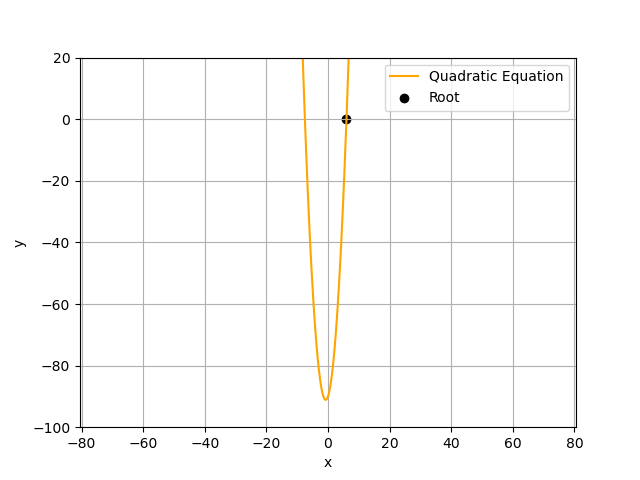
\includegraphics[width=0.7\columnwidth]{figs/graph.png}
   \caption{Objective Function with the minimum point}
   \label{label}
\end{figure}

\end{document}
